\documentclass[letterpaper,10pt]{article}

\usepackage{enumitem}
\usepackage{titling}
\usepackage{listings,listings-rust}
\usepackage{url}
\usepackage{soul}
\usepackage{hyperref}
\usepackage{setspace}
\usepackage{subfig}
\usepackage{sectsty}
\usepackage{pdfpages}
\usepackage{colortbl}
\usepackage{multirow}
\usepackage{multicol}
\usepackage{relsize}
\usepackage{amsmath}
\usepackage{wasysym}
\usepackage{fancyvrb}
\usepackage[yyyymmdd]{datetime}
\usepackage{amsmath,amssymb,amsthm,graphicx,xspace}
\usepackage[titlenotnumbered,noend,noline]{algorithm2e}
\usepackage[compact]{titlesec}
\usepackage{XCharter}
\usepackage[T1]{fontenc}
\usepackage[scaled]{beramono}
\usepackage[normalem]{ulem}
\usepackage{booktabs}
\usepackage{tikz}
\usetikzlibrary{arrows.meta,automata,shapes,trees,matrix,chains,scopes,positioning,calc,decorations.pathreplacing}
\tikzstyle{block} = [rectangle, draw, fill=blue!20, 
    text width=2.5em, text centered, rounded corners, minimum height=2em]
\tikzstyle{bw} = [rectangle, draw, fill=blue!20, 
    text width=4em, text centered, rounded corners, minimum height=2em]

\definecolor{namerow}{cmyk}{.40,.40,.40,.40}
\definecolor{namecol}{cmyk}{.40,.40,.40,.40}
\renewcommand{\dateseparator}{-}

\let\LaTeXtitle\title
\renewcommand{\title}[1]{\LaTeXtitle{\textsf{#1}}}

\lstset{basicstyle=\footnotesize\ttfamily,breaklines=true}

\newcommand{\CPP}{C\nolinebreak\hspace{-.05em}\raisebox{.4ex}{\tiny\bf +}\nolinebreak\hspace{-.10em}\raisebox{.4ex}{\tiny\bf +}}
\def\CPP{{C\nolinebreak[4]\hspace{-.05em}\raisebox{.4ex}{\tiny\bf ++}}}

\newcommand{\handout}[5]{
  \noindent
  \begin{center}
  \framebox{
    \vbox{
      \hbox to 5.78in { {\bf ECE459: Programming for Performance } \hfill #2 }
      \vspace{4mm}
      \hbox to 5.78in { {\Large \hfill #4  \hfill} }
      \vspace{2mm}
      \hbox to 5.78in { {\em #3 \hfill \today} }
    }
  }
  \end{center}
  \vspace*{4mm}
}

\newcommand{\lecture}[3]{\handout{#1}{#2}{#3}{Lecture#1}}
\newcommand{\tuple}[1]{\ensuremath{\left\langle #1 \right\rangle}\xspace}

\addtolength{\oddsidemargin}{-1.000in}
\addtolength{\evensidemargin}{-0.500in}
\addtolength{\textwidth}{2.0in}
\addtolength{\topmargin}{-1.000in}
\addtolength{\textheight}{1.75in}
\addtolength{\parskip}{\baselineskip}
\setlength{\parindent}{0in}
\renewcommand{\baselinestretch}{1.5}
\newcommand{\term}{Winter 2020}

\singlespace


\begin{document}

\lecture{23 --- GPU Programming Continued }{\term}{Jeff Zarnett}

\section*{GPUs: Heterogeneous Programming}

\section*{Host Code}
We've learned about how a kernel works and a bit about how to write one. The next part is the host code. Now, fortunately, we don't have to write the whole program in \CPP~ or C, even though the kernel has to be written in the CUDA variant. We're going to use the Rustacuda library from \url{https://github.com/bheisler/RustaCUDA}. That allows us to write code in Rust that interfaces with the GPU, and we can limit the interactions with unsafe code as much as possible.
 
We'll look at a quick example of launching a very simple kernel from the Rustacuda examples\footnote{\url{https://github.com/bheisler/RustaCUDA/blob/master/examples/launch.rs}}: 
\begin{lstlisting}[language=Rust]
#[macro_use]
extern crate rustacuda;

use rustacuda::prelude::*;
use std::error::Error;
use std::ffi::CString;

fn main() -> Result<(), Box<dyn Error>> {
    // Set up the context, load the module, and create a stream to run kernels in.
    rustacuda::init(CudaFlags::empty())?;
    let device = Device::get_device(0)?;
    let _ctx = Context::create_and_push(ContextFlags::MAP_HOST | ContextFlags::SCHED_AUTO, device)?;

    let ptx = CString::new(include_str!("../resources/add.ptx"))?;
    let module = Module::load_from_string(&ptx)?;
    let stream = Stream::new(StreamFlags::NON_BLOCKING, None)?;

    // Create buffers for data
    let mut in_x = DeviceBuffer::from_slice(&[1.0f32; 10])?;
    let mut in_y = DeviceBuffer::from_slice(&[2.0f32; 10])?;
    let mut out_1 = DeviceBuffer::from_slice(&[0.0f32; 10])?;
    let mut out_2 = DeviceBuffer::from_slice(&[0.0f32; 10])?;

    // This kernel adds each element in `in_x` and `in_y` and writes the result into `out`.
    unsafe {
        // Launch the kernel with one block of one thread, no dynamic shared memory on `stream`.
        let result = launch!(module.sum<<<1, 1, 0, stream>>>(
            in_x.as_device_ptr(),
            in_y.as_device_ptr(),
            out_1.as_device_ptr(),
            out_1.len()
        ));
        result?;
    }

    // Kernel launches are asynchronous, so we wait for the kernels to finish executing.
    stream.synchronize()?;

    // Copy the results back to host memory
    let mut out_host = [0.0f32; 20];
    out_1.copy_to(&mut out_host[0..10])?;
    out_2.copy_to(&mut out_host[10..20])?;

    for x in out_host.iter() {
        assert_eq!(3.0 as u32, *x as u32);
    }

    println!("Launched kernel successfully.");
    Ok(())
}
\end{lstlisting}

And the kernel it corresponds to is\footnote{\url{https://github.com/bheisler/RustaCUDA/blob/master/resources/add.cu}}:
\begin{lstlisting}[language=C]
extern "C" __constant__ int my_constant = 314;

extern "C" __global__ void sum(const float* x, const float* y, float* out, int count) {
    for (int i = blockIdx.x * blockDim.x + threadIdx.x; i < count; i += blockDim.x * gridDim.x) {
        out[i] = x[i] + y[i];
    }
}
\end{lstlisting}

\paragraph{Walk-through.} Let's look at all of the code in the example and
explain the terms. For a more detailed explanation of all the steps, see~\cite{cuda}.

One thing that we won't see is any explicit call to initialize the runtime. The CUDA runtime is automatically initialized when there's the first call into it. Thus, the first call might report errors that you wouldn't expect from that call, because they are really a setup problem on your system.

Right, in the example, we need to include the prelude for Rustacuda, just as we've seen previously for Rayon. This imports a bunch of commonly used types to save on having a lot of imports. 

First thing we have to do is initialize the API. This has to happen at the start of the program, so no sense in delaying it! At present, there are no flags defined so the call with \texttt{CudaFlags::empty()} is the only valid argument to the initialization function. 

Then we get a \textit{device}. The device is your graphics card or any other hardware that does the work. It's obviously possible to have more than one compute device, but we'll just take the first one. 

Next, in step 3, we request a \emph{context}. The context is described by the documents as analogous to a process. When we launch something within that context, it executes in there and has its own address space, and when the context is destroyed, all its resources are cleaned up. Each host thread may have one context. The call shown is ``create and push'' because a host thread has a stack of current contexts. We don't actually need the context for any of the later steps, but we just need to be in possession of one. In this simple example, stays in scope because everything happens in \texttt{main}. If you want more structure to your program, then you do have to ensure it doesn't go out of scope and get dropped, because it has to exist for the other functions to work. When it does get dropped, some cleanup actions take place, of course.

The next step is to create our \textit{module}. A module is technically a package of code and data to run on the device, but in this case it just really means our kernel. What we do here is read the compiled PTX code into a C-String, then create the module from that string. It's also possible to load from a file directly. 

Once we have created a module, we then create a \textit{stream}. The stream is where we assign work. You can think of it as being similar to a priority queue: you put items in there and work that is more important (lower priority number) can pre-empt work that is less important (higher priority number). Otherwise, work is done in the order it was scheduled, and tasks don't overlap. The stream is asynchronous, so once work has been assigned, it returns immediately. I'll point out that the Rustacuda implementation says you should set the \texttt{NON\_BLOCKING} flag to prevent synchronization with the NULL stream (the details of which we'll skip). 

There's one more step before launching the kernel; in step 5, we
create some \emph{data buffers}, which are used for moving data to and from the GPU. Remember, CUDA requires explicit communication, so whatever data want to provide as input has to be put into a buffer and then the buffer is transferred to the kernel. Whatever data comes as output will be transferred by the GPU into the output buffers we specify.

After all this setup, we can finally launch the kernel. This has to be done in an \texttt{unsafe} block, because the launch macro is unsafe (unfortunately). The good news is that the unsafe block is only the launch, limiting the area of extra scrutiny to something small. When we launch, we specify the kernel that's supposed to run as well as the arguments. Each buffer is converted using the \texttt{as\_device\_ptr()} so that the contents of the device buffer are provided. For scalar types like the count, no such conversion is necessary and we can just provide the value. Here, we specify the grid size and block size (1 each). We'll be returning to that subject a bit.

Great! We launched the kernel and sent it over to the GPU. This is an asynchronous process, so we could do more stuff here if we need. There's nothing else to do at the moment, so we'll wait for the items in the queue to complete by calling \texttt{stream.synchronize()}. Straightforward!

Finally, in the last step, we copy the items out of the buffer and back into host memory. Here, the example code checks that all the values are correct (3.0) and it is! Alright, we have a simple working example of how to setup, launch, and collect results from a CUDA computation!

\subsection*{N-Body Host Code}

Here's the corresponding host code for the N-Body problem where we saw the kernel last time. A lot of it will be the same as the example code, but there are some differences that are noteworthy. Let's get started.

\begin{lstlisting}[language=Rust]
#[macro_use]
extern crate rustacuda;
extern crate rustacuda_derive;
extern crate rustacuda_core;

use cuda_sys::vector_types::{float3, float4};
use rustacuda::prelude::*;
use std::error::Error;
use std::ffi::CString;
use rand::Rng;
use rustacuda_core::DeviceCopy;
use std::ops::Deref;

/* A Rustification by Jeff Zarnett of a past ECE 459 N-Body assignment that was
originally from GPU Gems, Chapter 31 and modified by Patrick Lam.
Then CUDA-fied by Jeff Zarnett using the Rustacuda library example code
 */

const NUM_POINTS: u32 = 100000;
const SPACE: f32 = 1000.0;

struct CudaFloat4(float4);
unsafe impl DeviceCopy for CudaFloat4 {}
impl Deref for CudaFloat4 {
    type Target = float4;

    fn deref(&self) -> &Self::Target {
        &self.0
    }
}
struct CudaFloat3(float3);
unsafe impl DeviceCopy for CudaFloat3 {}
impl Deref for CudaFloat3 {
    type Target = float3;

    fn deref(&self) -> &Self::Target {
        &self.0
    }
}

fn main() -> Result<(), Box<dyn Error>> {
    // Set up the context, load the module, and create a stream to run kernels in.
    rustacuda::init(CudaFlags::empty())?;
    let device = Device::get_device(0)?;
    let _ctx = Context::create_and_push(ContextFlags::MAP_HOST | ContextFlags::SCHED_AUTO, device)?;

    let initial_positions = initialize_positions();
    println! {"Initial positions:"}
    for pt in initial_positions.iter() {
        println! {"({}, {}, {}) [{}]", pt.x, pt.y, pt.z, pt.w};
    }
    let mut accelerations = initialize_accelerations();

    let ptx = CString::new(include_str!("../resources/nbody.ptx"))?;
    let module = Module::load_from_string(&ptx)?;
    let stream = Stream::new(StreamFlags::NON_BLOCKING, None)?;

    // Create buffers for data
    let mut points = DeviceBuffer::from_slice(initial_positions.as_slice())?;
    let mut accel = DeviceBuffer::from_slice(accelerations.as_slice())?;

    unsafe {
        // Launch the kernel with one block for each point, with 1 thread each, no dynamic shared memory on `stream`.
        let result = launch!(module.calculate_forces<<<NUM_POINTS, 1, 0, stream>>>(
            points.as_device_ptr(),
            accel.as_device_ptr(),
            points.len()
        ));
        result?;
    }

    // Kernel launches are asynchronous, so we wait for the kernels to finish executing.
    stream.synchronize()?;

    // Copy the results back to host memory
    accel.copy_to(&mut accelerations)?;

    println! {"Accelerations:"}
    for a in accelerations.iter() {
        println! {"({}, {}, {})", a.x, a.y, a.z};
    }
    Ok(())
}

fn initialize_positions() -> Vec<CudaFloat4> {
    let mut result: Vec<CudaFloat4> = Vec::new();
    let mut rng = rand::thread_rng();

    for _i in 0..NUM_POINTS {
        result.push(CudaFloat4 {
            0: float4 {
                x: rng.gen_range(0.0, SPACE),
                y: rng.gen_range(0.0, SPACE),
                z: rng.gen_range(0.0, SPACE),
                w: rng.gen_range(0.01, 100.0),
            }
        });
    }
    result
}

fn initialize_accelerations() -> Vec<CudaFloat3> {
    let mut result: Vec<CudaFloat3> = Vec::new();
    for _i in 0 .. NUM_POINTS {
        result.push(CudaFloat3 {
            0: float3 {
                x: 0f32,
                y: 0f32,
                z: 0f32,
            }
        });
    }
    result
}
\end{lstlisting}

We mentioned last time that in the kernel we can use vector types like \texttt{float4}. If we want to use those in Rust, we have to import them from a library (here cuda-sys) that isn't the same as the Rustacuda library\footnote{So at the time that I wrote this, I actually submitted an issue in the Rustacuda library to bring in support for this. Maybe by the time you are reading this, support has been added. I might even have found time to do it myself, should I finish all the course content and have time.}. This gives us the \texttt{float4} but there's a requirement of the Rustacuda library that any type that we want to send over to the kernel must have the trait \texttt{DeviceCopy}. Implementing the trait is promising that the type you have does not contain any pointers to host memory (so if you had a struct that contained a pointer to a buffer, this is not okay). That's because the pointer will be bogus when it is on the GPU device (they don't share memory). I also added the \texttt{Deref} trait which makes it so that the array of this type \texttt{CudaFloat4} will be easily converted to the type it contains \texttt{float4} when we operate on it. And the same for the \texttt{float3} type.


The other thing worth noting is that the calculation of forces kernel is invoked with a grid size of \texttt{NUM\_POINTS} and one thread per block. That is to say, there are \texttt{NUM\_POINTS} (100~000) chunks of work, and each chunk has one thread. If you get this wrong, the code doesn't work as expected: if you put in 1 and 1 for both of these values, then only the first acceleration will be calculated, because we said there's one chunk of work and it's one thread. But what we actually have asked for is to have \texttt{NUM\_POINTS} chunks and that will get it done.

When done, we copy the data out and print it and we're done! Below that, you an also see there's a little change to how the initial values are created in that we have to set the content of the \texttt{CudaFloat3/4} through parameter 0. 

\paragraph{Putting it to the test.}
That's great, but how much does it speed up? I ran this on ecetesla1 (because my laptop does not have the correct graphics card for this purpose), so I reran all the CPU benchmarks to have a fair comparison for what happens on the same machine. With 100~000 points:
\begin{itemize}
	\item \texttt{nbody} (sequential, no approximations): 40.3 seconds\vspace{-1em}
	\item \texttt{nbody-parallel} (parallel, no approximations): 5.3 seconds\vspace{-1em}
	\item \texttt{nbody-cuda} (parallel, no approximations): 9.5 seconds
\end{itemize}

Hey, wait a minute. That's worse than the CPU version. Uh, what's wrong here? My first theory was that 100~000 points is not enough to overcome the overhead of setup and transferring data to and from the device. This turned out to be incorrect (and it was painful to try the sequential version with more points). 

Eventually, I used a profiler (we'll come back to profiling shortly) and it told me that most of the time was going to the kernel execution of the \texttt{calculate\_forces} function. This convinced me that the problem was that I wasn't getting the most out of the GPU as I could be. I don't think there was anything terrible about the kernel itself, but I really wanted to go back to the question of the grids and blocks Here's a (sadly terrible quality) image from the CUDA docs that explains it~\cite{cuda}:
\begin{center}
	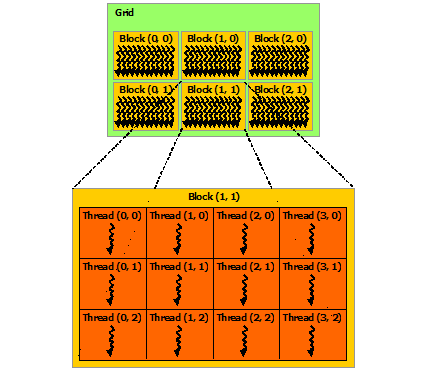
\includegraphics[width=0.5\textwidth]{images/grid-of-thread-blocks.png}
\end{center}

The documentation isn't super great about how grids and blocks work, unfortunately, and a lot of the guidance on the internet says is ``experiment and try'' (so helpful). The initial approach that I wrote had each work-item be its own block. That's inefficient, because we're not taking advantage of all the hardware that's available (the warp hardware). The advice that I can find says the number of threads per block should always be a multiple of 32 with a maximum of 512 (or perhaps 1024 with more modern devices). The second guidance I can find is that numbers like 256 and 128 are good ones to start with, and you can tweak it as you need. Then you have to adjust the grid size: divide the number of points by the threads per block to give the number of blocks. Here's the improved call:

\begin{lstlisting}[language=Rust]
        let result = launch!(module.calculate_forces<<<(NUM_POINTS/256) + 1, 256, 0, stream>>>(
            points.as_device_ptr(),
            accel.as_device_ptr(),
            points.len()
        ));
        result?;
\end{lstlisting}

I did have to add a +1 to the number of blocks, because 100~000 does not divide evenly by 256, and if you forget that then the last few of the accelerations are all zeros. But just running it as-is didn't work (and led to the kernel crashing. Why? Because the indexing strategy that I used contained only the reference to the block index \texttt{blockIdx.x}. That's fine in the scenario where every work-item gets its own block, but that's no longer the case now: 256 work-items (points) now share each block. Here's the adjusted kernel the calculates the correct index. 

\begin{lstlisting}[language=C++]
extern "C" __global__ void calculate_forces(const float4* positions, float3* accelerations, int num_points) {
    int idx = threadIdx.x + blockIdx.x * blockDim.x;
    if (idx >= num_points) {
        return;
    }
    float4 current = positions[idx];
    float3 acc = accelerations[idx];

    for (int i = 0; i < num_points; i++) {
        body_body_interaction(current, positions[i], &acc);
    }
    accelerations[idx] = acc;
}
\end{lstlisting}

The full version of the improved code is in the course repository as \texttt{nbody-cuda-grid}. But what you want to know is, did these changes work? Yes! It sped up the calculation to about 1.65 seconds (still with 100~000 points, still on the same server). Now that's a lot better! We are finally putting the parallel compute power of the GPU to good use and it results in an excellent speedup.

\bibliographystyle{alphaurl}
\bibliography{459}


\end{document}
